% Conclusion

\begin{frame}[c]
  \frametitle{Conclusion générale}

Les Frappes de Processus standard permettent une \tval{représentation atomique}\\
des réseaux de régulation biologique :
\begin{itemize}
  \item Analyse statique efficace existante
  \item Mais problèmes de décalage temporel
  \item Limites de modélisation
\end{itemize}

\medskip
\tval{Nouvelles sémantiques} pour augmenter l'expressivité :
\begin{itemize}
  \item Correction du décalage temporel \f expressivité strictement plus forte
  \item Possibilité de simuler des paramètres temporels
  \item Nouveaux liens avec d'autres formalismes (Thomas, RdP, etc.)
\end{itemize}

\medskip
Nouvelle \tval{analyse statique} sous forme canonique :
\begin{itemize}
  \item analyse efficace de propriétés dynamiques
  \item Nouveau type de propriétés : activation simultanée
\end{itemize}

% 
% 
% Process Hitting: an atomistic modeling with powerful static analysis
% 
% \medskip
% \begin{enumerate}[1.]
%   \item Stochastic parameters:
%     \begin{itemize}
%       \item To model systems with chronometric features
%       \item \tval{Continuous time}
%       \item But \tval{hard to analyze}
%     \end{itemize}
%   \item Classes of priorities:
%     \begin{itemize}
%       \item Allows to reproduce the same behaviors
%       \item Efficient \tval{static analysis}
%       \item But the translation to canonical form faces \tval{combinatorial explosion}
%     \end{itemize}
%   \item Neutralizing edges:
%     \begin{itemize}
%       \item Alternative to priorities
%       \item Closer to reality in some cases
%       \item \tval{Lighter translation} to canonical form
%     \end{itemize}
% \end{enumerate}
% 
% \vfill
% \Large
% \begin{flushright}
%   \tval{Thank you}\hspace{1cm}~
% \end{flushright}
% \vfill

\end{frame}



\begin{frame}[c]
  \frametitle{Ouvertures et perspectives}

Pistes d'\tval{exploitation} :
\begin{itemize}
  \item Modélisation et analyse de bases de données complètes
  \item Étude de comportements incontrôlables, de perturbations ponctuelles
  \item Recherche de propriétés intéressantes (attracteurs, oscillations...)
\end{itemize}

\medskip
Enrichissement de l'\tval{analyse statique} :
\begin{itemize}
  \item Raffinement pour réduire l'ensemble des cas non-conclusifs
  \item Utilisation de méthodes dérivées utilisant le graphe de causalité locale
  \item Développement de nouvelles propriétés (logiques temporelles, compteurs...)
\end{itemize}

\medskip
Enrichissement des \tval{capacités de représentation} :
\begin{itemize}
  \item Classes de priorités dynamiques
  \item Actions gardées ou portes logiques complexes
  \item Outils de vérification et correction (logique de Hoare)
\end{itemize}

\end{frame}



\begin{frame}[c]
  \frametitle{Participation et Collaborations}

Participation au projet \tval{ANR blanc BioTempo} (mars 2011 -- août 2014) :
\begin{center}
« Représentations à l’aide de langage, de temps et de modèles hybrides\\
pour l’analyse de modèles incomplets en biologie moléculaire »
\end{center}

%\tval{Inoue Laboratory} (NII, Sokendai): Constraint Programming, Systems Biology

%\tval{MeForBio} (IRCCyN, ÉCN): Formal Methods for Bioinformatics

%\tval{AMIB} (LIX, Polytechnique): Algorithms and Models for Integrative Biology

\bigskip\footnotesize
\begin{center}
  $\left.\text{\begin{tabular}{ccc}
      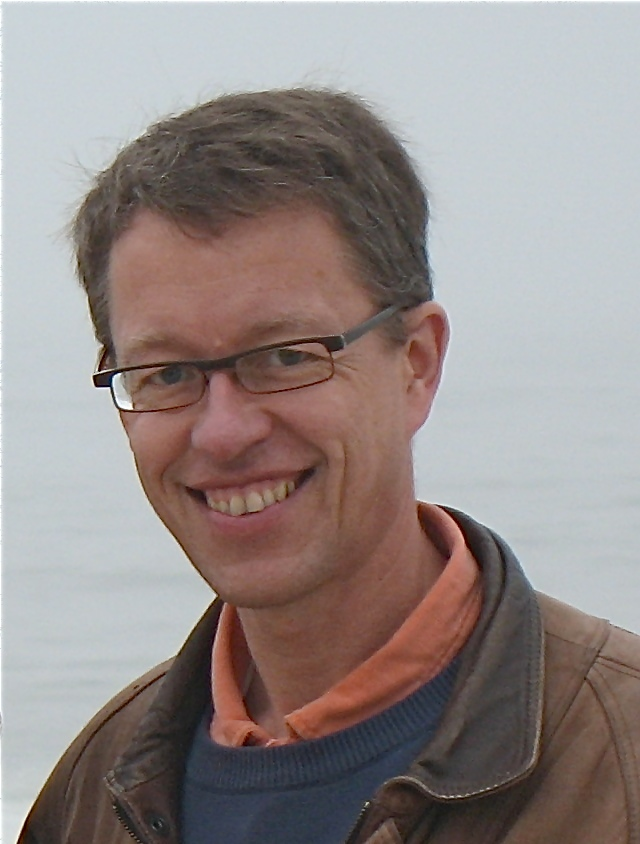
\includegraphics[height=1.5cm]{figs/Olivier.jpg}
    & 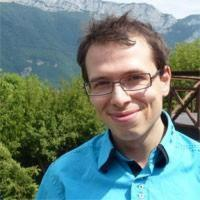
\includegraphics[height=1.5cm]{figs/Morgan.jpg} \\
      \tval{Olivier ROUX} & \tval{Morgan MAGNIN} \\
      Professeur \& chef d'équipe & Maître de conférences
  \end{tabular}}\right\}$ %\text{\tval{MeForBio}}$%}
  \parbox{2cm}{\tval{MeForBio}\\IRCCyN\\(Nantes, France)}

  \vspace*{3em}
  $\left.\text{\begin{tabular}{c}
    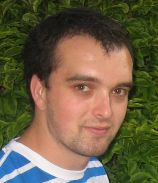
\includegraphics[height=1.5cm]{figs/Loic.jpg} \\ \tval{Loïc PAULEVÉ} \\ Chargé de recherche CNRS
  \end{tabular}}\right\}$%\text{\tval{AMIB}}$
  \parbox{1.5cm}{\tval{Bioinfo/AMIB}\\LRI\\(Orsay, France)}
  \hspace*{3em}
  $\left.\text{\begin{tabular}{c}
    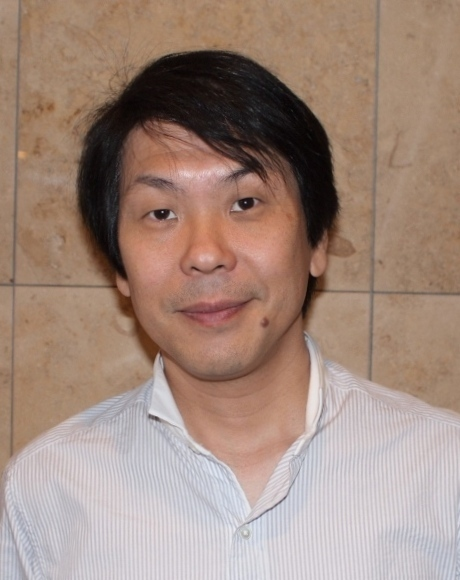
\includegraphics[height=1.5cm]{figs/Inoue-sensei.jpg} \\ \tval{Katsumi INOUE} \\ Professeur \& chef d'équipe
  \end{tabular}}\right\}$%\text{\tval{Inoue Laboratory}}$
  \parbox{1.5cm}{\tval{Inoue Lab.}\\NII\\(Tokyo, Japon)}
\end{center}

\end{frame}
